\documentclass{standalone}
\usepackage{tikz}
\usepackage{pgfplots}
\usetikzlibrary{patterns,decorations.markings,backgrounds}
\usetikzlibrary{arrows.meta}

% change font for specific paper
\usepackage{newtxtext,newtxmath}
\usepgfplotslibrary{colorbrewer,colormaps}

\pgfplotsset{compat=1.18}

% The figure's natural width (measure once, then set here)
\pgfplotsset{colormap/RdBu}

\def\tikzfontscale{12.08/7.85} % This will be computed by tikz-fontscale.sty

\begin{document}
\begin{tikzpicture}

	% import .png figure
	\draw[ultra thick] (-6.04, -2.8) -- (-5.3, -2.45) -- (-5.25, -2.98) -- (-2.85, -1.85) -- (-2.85, -1.3) -- (6.04, 2.66);
	\draw[ultra thick] (-5.25, -3) -- (-5.6, -2.6);
	\draw[ultra thick] (-6.04, -2.15) -- (-5.73,-2.03);
	\draw[ultra thick] (-5.38,-2.37) -- (-3.33,-1.45) --(-3.33,-1) -- (5.95,2.95);

	\draw[ultra thick] (-5.29, -2.44)-- (-5.75,-2.03);

	\node[inner sep=0pt] (gap) at (0,0){
		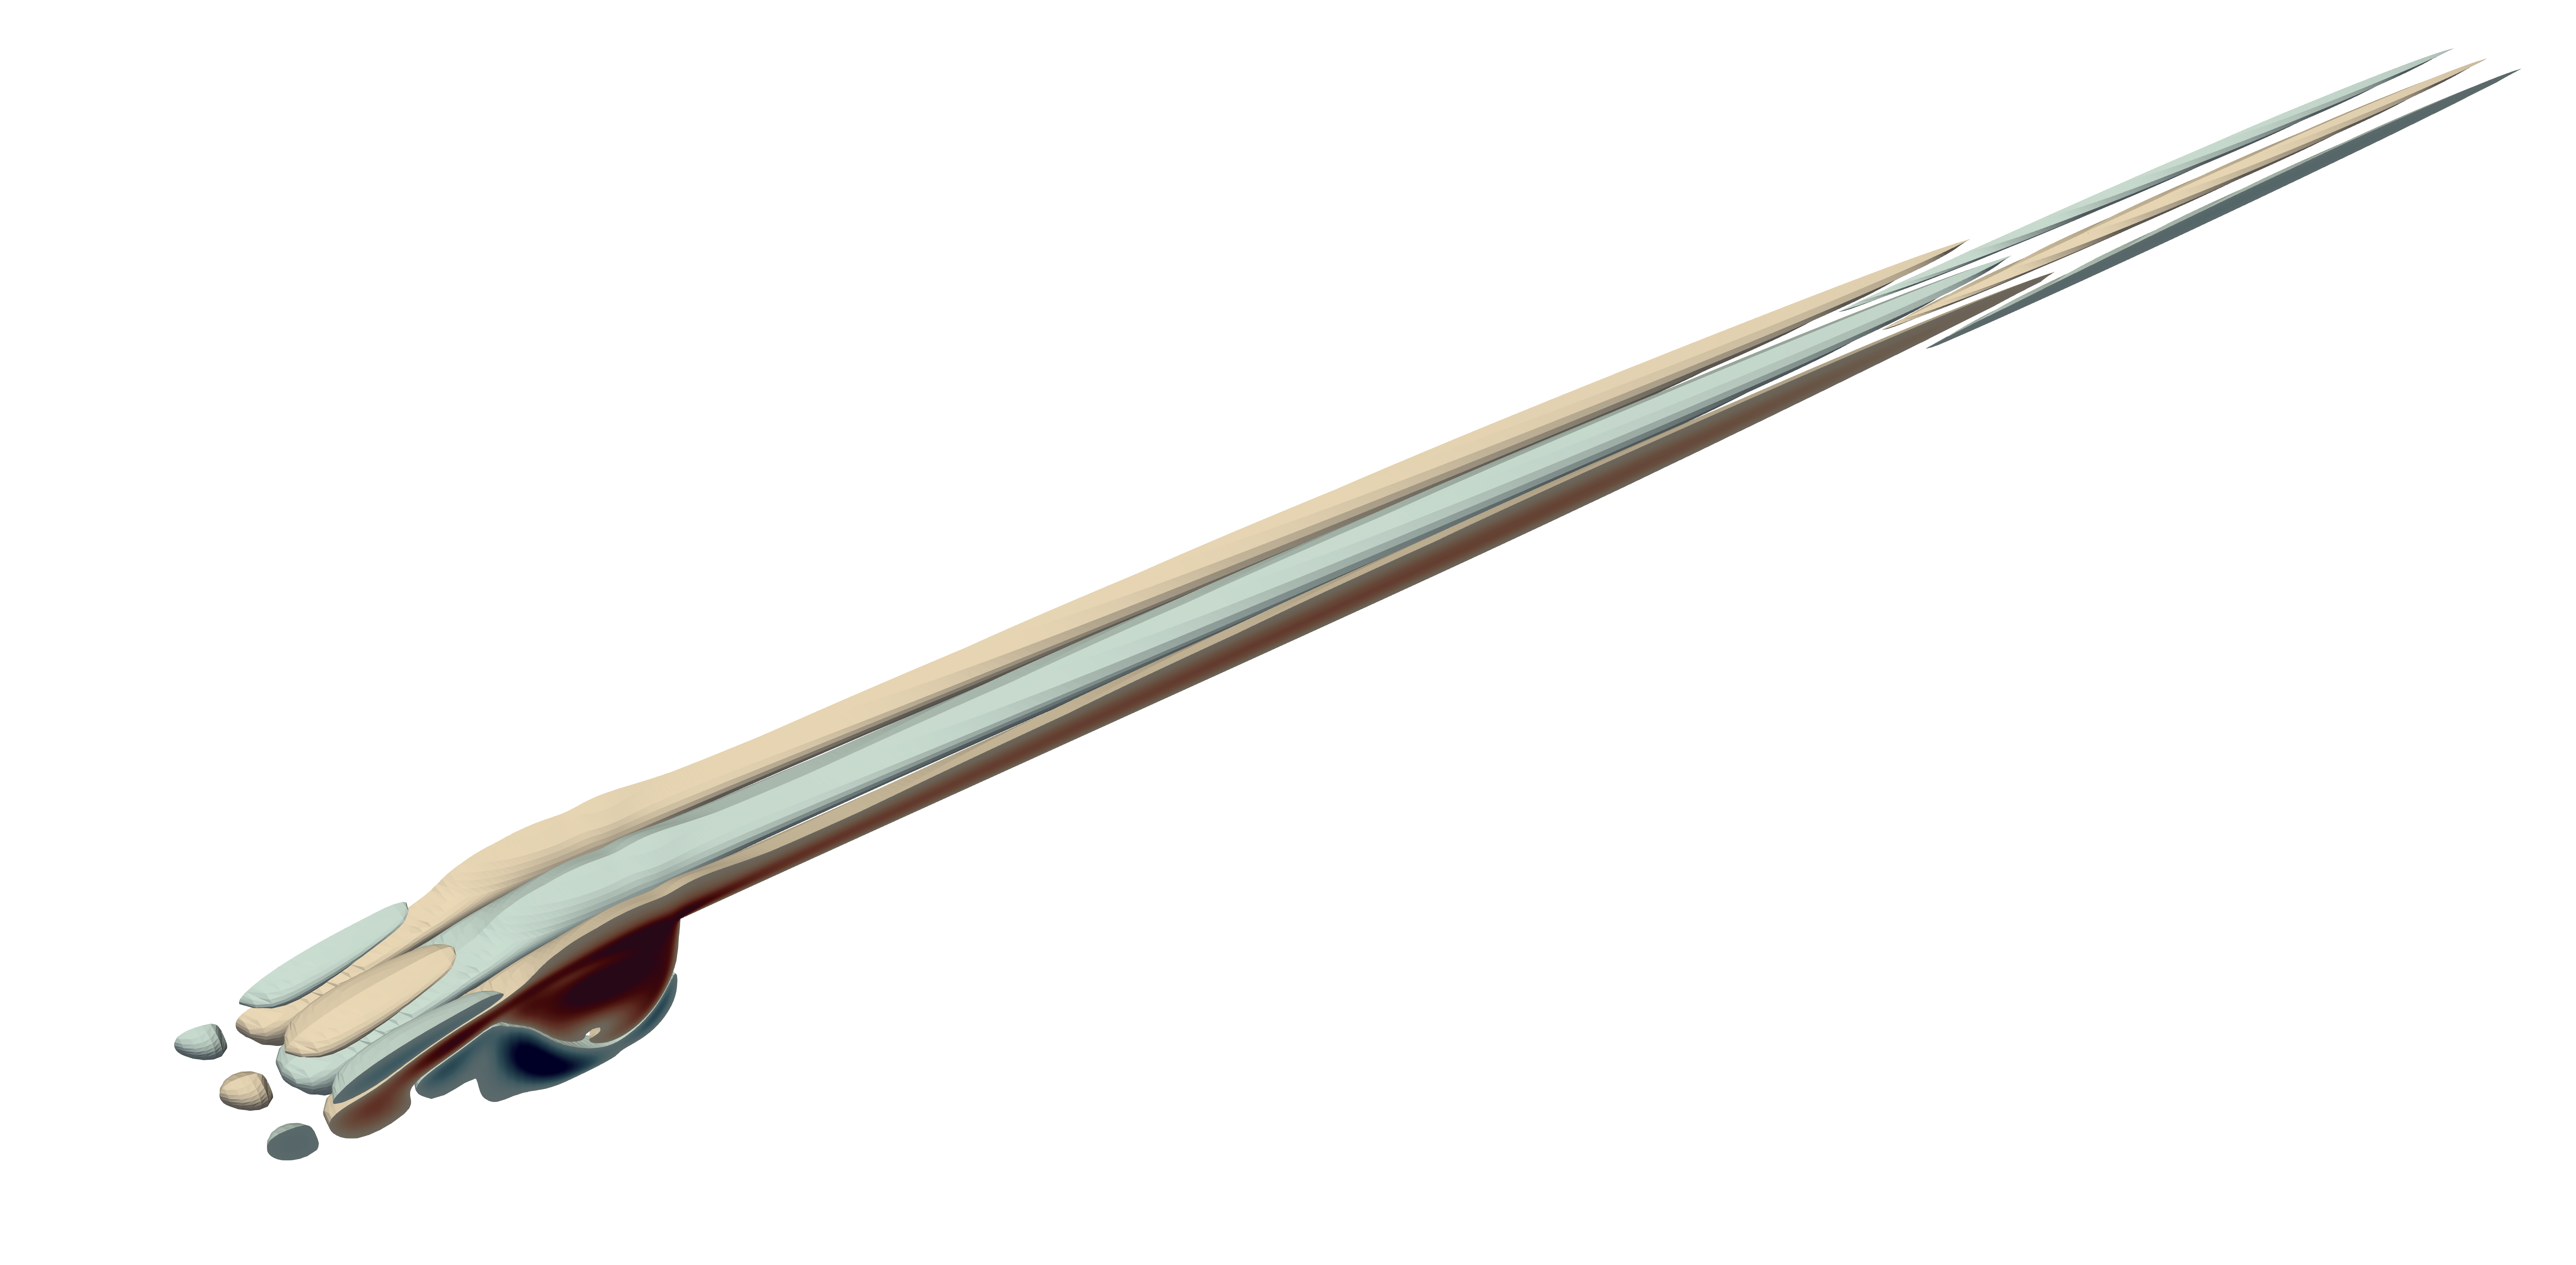
\includegraphics[width=\textwidth]{d4w143dmode.png}
	};

	\pgfplotscolorbardrawstandalone[
		colormap={example}{
				indices of colormap=(\pgfplotscolormaplastindexof{RdBu},...,0 of RdBu), % inversion of RdBu -> BuRd
			},
		point meta min=-0.02,
		point meta max=0.02,
		colorbar horizontal,
		samples=200,
		scaled x ticks=false,
		colorbar style={
				xtick={-0.02, -0.01, 0, 0.01, 0.02},
			xticklabel style={
						font=\small,
						scale=\tikzfontscale,
					},
				xticklabels={$-0.02$, $-0.01$, $0$, $0.01$, $0.02$},
				xlabel={$u'$},
				xlabel style={
					font=\small,
						scale=\tikzfontscale,
					},
				at={(gap.south)},
				yshift=-0.2cm,
				anchor=center,
				width=7cm,
				height=0.45cm,
				xtick pos=lower,
				xtick style={black, line width=0.8pt},
				tickwidth=3pt,
				axis line style={line width=0.8pt}
			},
	]
\end{tikzpicture}
\end{document}
